\section{Modellierung}

\begin{defi}{Modellierung}
    \emph{Modellierung} übersetzt ein reales Problem (Szenario/Mini-Welt, z.B. die lesenswerten Artikel) in eine \enquote{bearbeitbare} Version, das Modell, um final ein Ergebnis (Datenbankentwurf) systematisch zu entwickeln.

    Ein Modell sollte
    \begin{itemize}
        \item vollständig,
        \item korrekt,
        \item minimal,
        \item verständlich und
        \item erweiterbar
    \end{itemize}
    sein.
\end{defi}

\begin{defi}{ANSI/SPARC-Architektur}
    Die \emph{ANSI-SPARC-Architektur} (auch Drei-Schema-Architektur, Drei-Ebenen-Architektur oder Drei-Ebenen-Schema-Architektur) beschreibt die grundlegende Trennung verschiedener Beschreibungsebenen für Datenbankschemata.

    Die drei Ebenen sind:
    \begin{itemize}
        \item Die \emph{externe Ebene}, die den Benutzern und Anwendungen individuelle Benutzersichten bereitstellt. Beispiele: Formulare, Masken-Layouts, Listen, Schnittstellen.
        \item Die \emph{konzeptionelle Ebene}, in der beschrieben wird, welche Daten in der Datenbank gespeichert sind, sowie deren Beziehungen zueinander. Designziel ist hier eine vollständige und redundanzfreie Darstellung aller zu speichernden Informationen.
              Hier findet die Normalisierung des relationalen Datenbankschemas statt.
        \item Die \emph{interne Ebene} (auch physische Ebene), die die physische Sicht der Datenbank im Computer darstellt.
              In ihr wird beschrieben, wie und wo die Daten in der Datenbank gespeichert werden.
              Designziel ist hier ein effizienter Zugriff auf die gespeicherten Informationen.
              Das wird meistens nur durch eine bewusst in Kauf genommene Redundanz erreicht (z. B. im Index werden die gleichen Daten gespeichert, die auch schon in der Tabelle gespeichert sind).
    \end{itemize}

    Die Vorteile des Drei-Ebenen-Modells sind:
    \begin{itemize}
        \item Physische Datenunabhängigkeit: Die interne Ebene ist von der konzeptionellen und externen Ebene getrennt. Physische Änderungen, z. B. des Speichermediums oder des Datenbankprodukts, wirken sich nicht auf die konzeptionelle oder externe Ebene aus.
        \item Logische Datenunabhängigkeit: Die konzeptionelle und die externe Ebene sind getrennt.
              Dies bedeutet, dass Änderungen an der Datenbankstruktur (konzeptionelle Ebene) keine Auswirkungen auf die externe Ebene, also die Masken-Layouts, Listen und Schnittstellen haben.
    \end{itemize}
\end{defi}

\subsection{Entity-Relationship-Modell}

\begin{defi}{Entity-Relationship-Modell}
    Das \emph{Entity-Relationship-Modell} (kurz \emph{ER-Modell}) dient dazu, im Rahmen der semantischen Datenmodellierung den in einem gegebenen Kontext (z. B. einem Projekt zur Erstellung eines Informationssystems) relevanten Ausschnitt der realen Welt zu bestimmen und darzustellen.

    Grundlage der Entity-Relationship-Modelle ist die Typisierung von Objekten, ihrer Beziehungen untereinander und der über sie zu führenden Informationen („Attribute“).
\end{defi}

\subsubsection{Chen-Notation}

\begin{defi}{Chen-Notation}
    Die \emph{Chen-Notation} ist eine grafische Notation für Entity-Relationship-Modelle.

    Angegeben in der grafischen Darstellung werden die:
    \begin{itemize}
        \item Entitätstypen bzw. Klassen
        \item Kardinalitäten
        \item Beziehungstypen
    \end{itemize}

    Im Folgenden beziehen wir uns bis auf weiteres auf die Chen-Notation.
\end{defi}

\begin{defi}{Entität (Chen-Notation)}
    \begin{wrapfigure}{r}{0.25\textwidth}
        \begin{center}
            
\includegraphics[width=0.2\textwidth]{includes/figures/definition_entity_relationship_model_entity.pdf}
        \end{center}
    \end{wrapfigure}
    Eine \emph{Entität (\enquote{Entity})} $e$ beschreibt ein individuell identifizierbares Objekt der Wirklichkeit.
    Sie ist damit vergleichbar mit einer Objektinstanz und entspricht einem einzelnen Datensatz in einer Datenbank, z.B. das Pokémon \emph{Glumanda} oder die Attacke \emph{Flammenwurf}.
\end{defi}

\begin{defi}{Entitätstyp}
    Ein \emph{Entitätstyp (\enquote{Entity-Set})} beschreibt eine Menge $E$ von Entitäten $e \in E$ mit gleichen Eigenschaften (Klassifikation), z.B. \enquote{Pokémon}.
    Hier liegt eine Betrachtung als Menge von Objekten zugrunde.

    Ein Entitätstyp ist vergleichbar mit einer Klassenbeschreibung und entspricht damit häufig einer Tabelle in einer relationalen Datenbank, hierbei sind die Spalten die Attribute.
\end{defi}

\begin{defi}{Attribut (Chen-Notation)}
    \begin{wrapfigure}{r}{0.25\textwidth}
        \begin{center}
            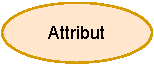
\includegraphics[width=0.2\textwidth]{includes/figures/definition_entity_relationship_model_attribute.pdf}
        \end{center}
    \end{wrapfigure}
    Eine \emph{Attribut (\enquote{Attribute})} definiert, was über eine Entität (im Kontext) von Interesse ist.
    Eine Entität $e$ ist durch die Werte ihrer Attribute charakterisiert und ein Entitätstyp $E$ durch die Attribute selber.

    Jedem Attribut $A$ ist ein Datentyp $T$ und damit implizit oder auch explizit ein Wertebereich $D$ (\enquote{Domain}) zugeordnet, der festlegt, welche Attributwerte zulässig sind\footnote{Wir schreiben: $A \in D$ oder $A:D$ bzw. $A:T$.}, z.B. \emph{Größe} und \emph{Gewicht} des Pokémon Glumanda vom Typ \texttt{float}, die \emph{Stärke} und \emph{Genauigkeit} der Attacke Flammenwurf vom Typ \texttt{int}.

    Besonders ist der Nullwert \texttt{NULL}.
    Das ist ein spezieller Attributwert, dessen Bedeutung variiert, d.h. z.B. ist der Wert unbekannt oder noch nicht festgelegt oder nicht möglich.
    \texttt{NULL} kann, muss aber nicht, im Wertebereich liegen.

    Wir notieren $E[A_1 : D_1, A_2 : D_2, \ldots, A_n : D_n]$ für einen Entitätstyp $E$ mit den Eigenschaften $A_1, \ldots, A_n$.
    Wertebereiche bzw. Typen werden, wenn nicht relevant, auch ausgelassen.

    $W(D)$ bezeichnet alle real existierenden Werte der Domain $D$ in einer Datenbank.
\end{defi}

\begin{defi}{Zusammengesetztes Attribut (Chen-Notation)}
    \begin{wrapfigure}{r}{0.35\textwidth}
        \begin{center}
            %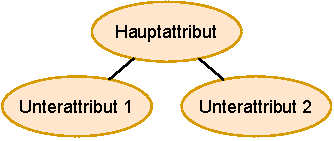
\includegraphics[width=0.4\textwidth]{includes/figures/definition_entity_relationship_model_attribute_combined.pdf}
            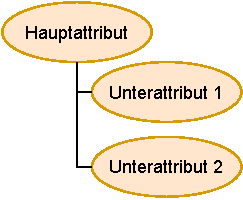
\includegraphics[width=0.3\textwidth]{includes/figures/definition_entity_relationship_model_attribute_combined_alt.pdf}
        \end{center}
    \end{wrapfigure}
    \emph{Zusammengesetzte Attribute} haben selbst Attribute, z.B.
    \begin{center}
        \texttt{Typ: [Primärtyp: char(30), Sekundärtyp: char(30)]}
    \end{center}

    Die Domain für ein zusammengesetztes Attribut $A$ mit Unterattributen $A_1, \ldots, A_n$ ist dann gegeben mit:
    \[
        A: [A_1 : D_2, \ldots, A_n:D_n]: D_1 \times \ldots \times D_n
    \]
\end{defi}

\begin{defi}{Mehrwertiges Attribut (Chen-Notation)}
    \begin{wrapfigure}{r}{0.25\textwidth}
        \begin{center}
            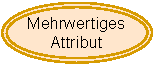
\includegraphics[width=0.2\textwidth]{includes/figures/definition_entity_relationship_model_attribute_multivalue.pdf}
        \end{center}
    \end{wrapfigure}
    Ein \emph{mehrwertiges Attribut} kann mehrere Ausprägungen bzw. Werte haben, z.B.
    \begin{center}
        \texttt{Attacke: \{char(255)\}}
    \end{center}

    Die Domain für ein mehrwertiges Attribut ist dann gegeben mit
    \[
        E : \{A\}
    \]
\end{defi}

\begin{defi}{Schlüsselkandidat (Chen-Notation)}
    \begin{wrapfigure}{r}{0.25\textwidth}
        \begin{center}
            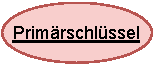
\includegraphics[width=0.2\textwidth]{includes/figures/definition_entity_relationship_model_attribute_primary.pdf}
        \end{center}
    \end{wrapfigure}
    Ein \emph{Schlüsselkandidat}, oder kurz Schlüssel (\enquote{key}), ist ein einwertiges Attribut oder eine Attributkombination, die jede Entität eindeutig identifiziert.

    Es ist möglich, dass mehrere Schlüsselkandidaten existieren.

    Der sogenannte \emph{Primärschlüssel} ist ein ausgewählter Schlüsselkandidat.
    Seine Primärschlüssel-attribute werden im ER-Diagramm durch Unterstreichung gekennzeichnet.

    Formal wird ein Primärschlüssel wie folgt dargestellt:
    \begin{center}
        \texttt{E: <[Attribute], \{Primärschlüssel\}>}
    \end{center}
    z.B.:
    \begin{center}
        \texttt{Pokemon: <[ID, Name, Typ: [Primärtyp, Sekundärtyp], \{Attacke: Name\}], \{ID\}>}
    \end{center}
\end{defi}

\begin{defi}{Relation (Chen-Notation)}
    \begin{wrapfigure}{r}{0.25\textwidth}
        \begin{center}
            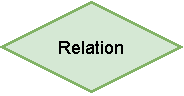
\includegraphics[width=0.2\textwidth]{includes/figures/definition_entity_relationship_model_relation.pdf}
        \end{center}
    \end{wrapfigure}
    Eine \emph{Relation (\enquote{Relationship})} erzeugt eine Verknüpfung bzw. einen Zusammenhang zwischen zwei oder mehreren Entitäten.

    Eine Relationship-Menge $R$ entspricht einer mathematischer Relation zwischen $n$ Entity-Mengen $E_i$:
    \[
        R \subseteq E_1 \times \ldots \times E_n \qquad (\text{häufig} \ n \in \{2, 3\})
    \]
    Eine Relation gibt an, ob eine Entität $e_1 \in E_1$ zu einer anderen Entität $e_2 \in E_2$ in Beziehung steht oder nicht, d.h.
    \[
        (e_1, e_2) \in R \quad \text{bzw.} \quad (e_1, e_2) \notin R
    \]

    z.B. gilt also:
    \[
        \text{Pokémon Pikachu \emph{lernt} die Attacke Donner} \ \iff \ (\text{Pikachu}, \, \text{Donner}) \in \text{lernt}
    \]
    \[
        \text{Pokémon Pikachu \emph{lernt} die Attacke Glut \emph{nicht}} \ \iff \ (\text{Pikachu}, \, \text{Glut}) \notin \text{lernt}
    \]

    Relationen können genau wie Entitäten Attribute besitzen.

    Sei $A = [A_1 : D_1, \ldots, A_m : D_m]$ ein Tupel mit $m$ Attributen $A = A_1, \ldots, A_m$ und $E_1, \ldots, E_n$ eine Menge von Entitätstypen.
    Dann ist
    \[
        R \subseteq E_1 \times \ldots \times E_n \times D_1 \times \ldots \times D_m
    \]
    eine mit $A$ attributierte Relation.

    Relationen können genauso gut auch reflexiv sein.
    Das kann im Diagramm mit Pfeilen verdeutlicht werden.
\end{defi}

\begin{defi}{Kardinalität (Chen-Notation)}
    \begin{wrapfigure}{r}{0.45\textwidth}
        \begin{center}
            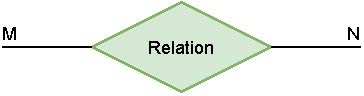
\includegraphics[width=0.4\textwidth]{includes/figures/definition_entity_relationship_model_cardinality.pdf}
        \end{center}
    \end{wrapfigure}
    Die \emph{Kardinalität} gibt an, zu wie vielen Elementen ein Element in Beziehung steht.

    Es gibt grundsätzlich folgende Abbildungsbeziehungen zwischen Entity-Mengen in der Chen-Notation:\footnote{In der Chen-Notation können $1$, $n$ und $m$ auch $0$ meinen!}
    \begin{itemize}
        \item \emph{1:1} (One-to-One)
        \item \emph{1:n} (One-to-Many) bzw. \emph{n:1} (Many-to-One)
        \item \emph{m:n} (Many-to-Many)
    \end{itemize}

    Die Kardinalität ergibt sich im Wesentlichen aus den Anforderungen und bestimmt ganz maßgeblich den Datenbankentwurf.
\end{defi}

\newpage

\begin{example}{1:1 Relation (Chen-Notation)}
    In Pokémon verleiht im Laufe des Spiels jede \emph{Arena} genau einen \emph{Orden}.

    Damit gilt:
    \begin{center}
        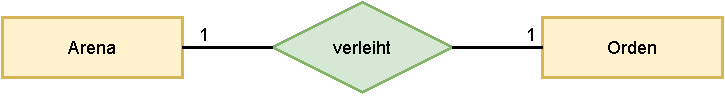
\includegraphics[width=0.7\linewidth]{includes/figures/example_entity_relationship_modell_chen_one_to_one.pdf}
    \end{center}
\end{example}

\begin{example}{1:n Relation (Chen-Notation)}
    In Pokémon hat jede \emph{Arena} mindestens einen, manchmal aber auch mehrere \emph{Arenaleiter}.

    Damit gilt:
    \begin{center}
        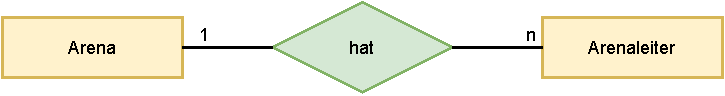
\includegraphics[width=0.7\linewidth]{includes/figures/example_entity_relationship_modell_chen_one_to_many.pdf}
    \end{center}
\end{example}

\begin{example}{n:1 Relation (Chen-Notation)}
    In Pokémon ist jede \emph{Attacke} von genau einem \emph{Typ}.

    Natürlich können aber mehrere \emph{Attacken} auch vom gleichen \emph{Typ} sein.

    Damit gilt:
    \begin{center}
        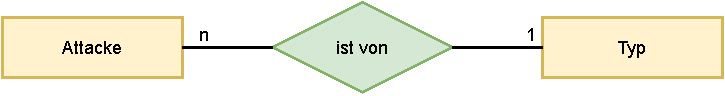
\includegraphics[width=0.7\linewidth]{includes/figures/example_entity_relationship_modell_chen_many_to_one.pdf}
    \end{center}
\end{example}

\begin{example}{m:n Relation (Chen-Notation)}
    In Pokémon kann jedes \emph{Pokémon} einige \emph{Attacken} lernen.

    Die selbe \emph{Attacke} kann aber gleichzeitig von mehreren \emph{Pokémon} erlernt werden.

    Damit gilt:
    \begin{center}
        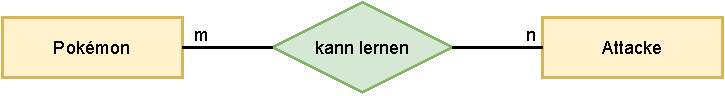
\includegraphics[width=0.7\linewidth]{includes/figures/example_entity_relationship_modell_chen_many_to_many.pdf}
    \end{center}
\end{example}

\begin{example}{Entity-Relationship-Modell (Chen-Notation)}
    \begin{center}
        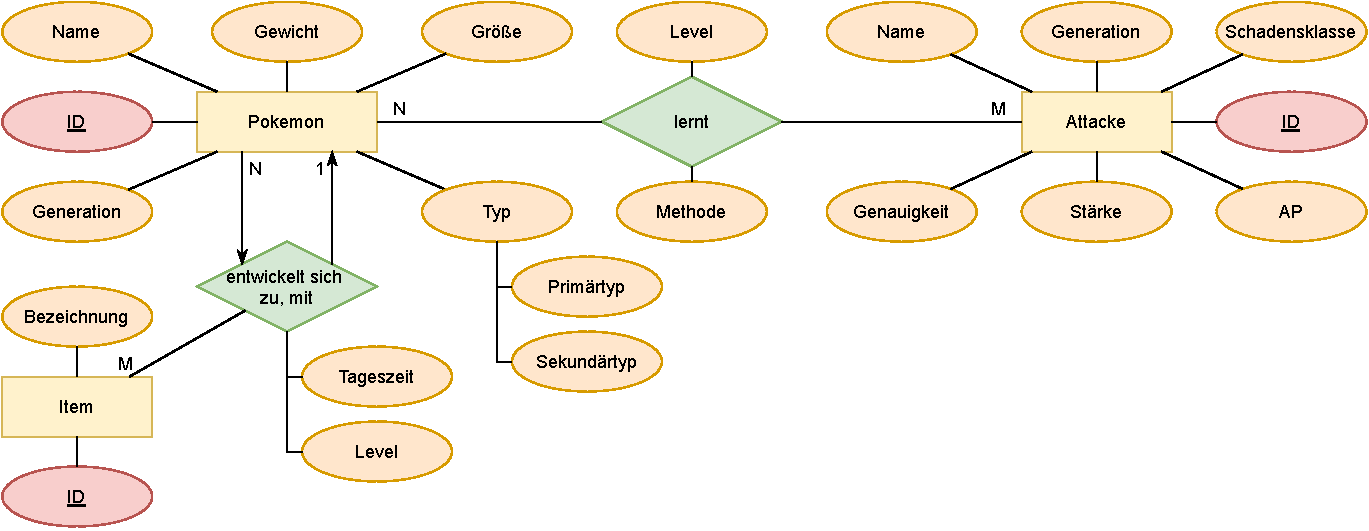
\includegraphics[width=\linewidth]{includes/figures/example_entity_relationship_modell_full.pdf}
    \end{center}
\end{example}

\begin{defi}{Existenzabhängiger Entitätstyp}
    \begin{wrapfigure}{r}{0.65\textwidth}
        \begin{center}
            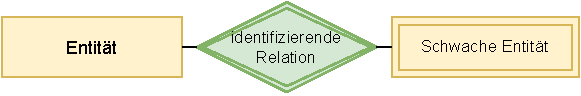
\includegraphics[width=0.6\textwidth]{includes/figures/definition_entity_relationship_model_entity_weak.pdf}
        \end{center}
    \end{wrapfigure}
    Die Grundidee von \emph{existenzabhängigen Entitätstypen} ist, dass sie nur in Verbindung mit anderen Entitäten existieren\footnote{vergleichbar mit der UML-Komposition}.

    Ein existenzabhängiger Entitätstyp hat keinen eigenen Schlüsselkandidaten, sondern wird über die Beziehung zur übergeordneten Entität identifiziert, z.B. über eine Kombination von Attributen.
\end{defi}

\begin{example}{Existenzabhängiger Entitätstyp}
    In Pokémon verleiht im Laufe des Spiels jede \emph{Arena} genau einen \emph{Orden}.

    Wir können das bisherige Beispiel insoweit verbessern, dass wir erkennen, dass ein spezieller Orden nicht ohne die jeweilige Arena existieren kann, bzw. wenn eine Arena aus der Datenbank gelöscht wird, der Orden ebenfalls gelöscht wird.

    Damit gilt:
    \begin{center}
        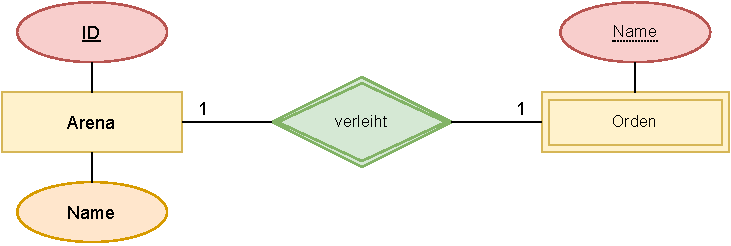
\includegraphics[width=0.7\linewidth]{includes/figures/example_entity_relationship_modell_entity_weak.pdf}
    \end{center}
\end{example}

\subsubsection{Min-Max-Notation}

\begin{defi}{Min-Max-Notation}
    \begin{wrapfigure}{r}{0.65\textwidth}
        \begin{center}
            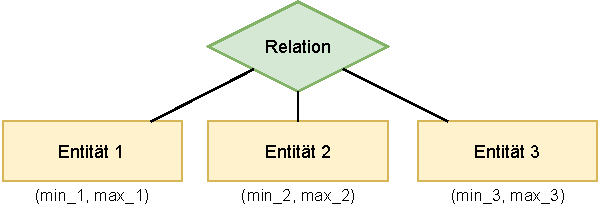
\includegraphics[width=0.6\textwidth]{includes/figures/definition_entity_relationship_min_max.pdf}
        \end{center}
    \end{wrapfigure}
    Ein Nachteil der Chen-Notation ist, dass die Angaben der Kardinalität sehr ungenau sind.

    Als Verbesserung wird die \emph{Min-Max-Notation} vorgeschlagen.
    In der Min-Max-Notation wird angegeben, wieviele Relationen minimal bzw. maximal möglich sein sollen.

    Für jeden an einer Relation beteiligten Entitätstypen $E_k$ wird angegeben, wie oft eine Entität minimal und maximal in der Relation enthalten sein darf.\footnote{
        Die Min-Max-Notation unterscheidet sich grundlegend von den anderen Notationsformen im Hinblick auf die Bestimmung der Kardinalität und die Position, an der die Häufigkeitsangabe im ER-Diagramm vorgenommen wird.

        Bei allen anderen Notationen wird die Kardinalität eines Beziehungstyps dadurch bestimmt, dass für eine Entität des einen Entitätstyps nach der Anzahl der möglichen beteiligten Entitäten des anderen Entitätstyps gefragt wird.

        Bei der Min-Max-Notation hingegen ist die Kardinalität anders definiert.
        Hierbei wird für jeden der an einem Beziehungstyp beteiligten Entitätstyp nach der kleinst- und größtmöglichen Anzahl der Beziehungen gefragt, an denen eine Entität des jeweiligen Entitätstyps beteiligt ist.

        Das jeweilige Min-Max-Ergebnis wird bei dem Entitätstyp notiert, für den die Frage gestellt wurde.
    }

    Sei $R \subseteq E_1 \times \ldots \times E_n$ und die Projektion auf das $k$-te Element bzw. die Anzahl eines Wertes an $k$-ter Stelle definiert durch
    \[
        \proj_k(e_1, \ldots, e_k, \ldots, e_n) = e_k
    \]
    \[
        \cnt_k(e) = \abs{ \{ r \in R \mid \proj_k(r) = e \} }
    \]
    dann muss für alle $k$ gelten:
    \[
        \forall e_k \in E_k : {\min}_k \leq \cnt_k(e_k) \leq {\max}_k
    \]
\end{defi}

\newpage

\begin{example}{1:1 Relation (Min-Max-Notation)}
    In Pokémon verleiht im Laufe des Spiels jede \emph{Arena} genau einen \emph{Orden}.

    Damit gilt:
    \begin{center}
        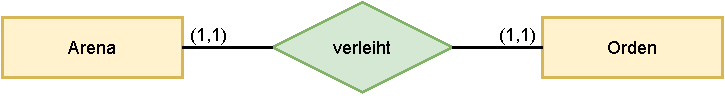
\includegraphics[width=0.7\linewidth]{includes/figures/example_entity_relationship_modell_min_max_one_to_one.pdf}
    \end{center}
\end{example}

\begin{example}{1:n Relation (Min-Max-Notation)}
    In Pokémon hat jede \emph{Arena} mindestens einen, manchmal aber auch mehrere \emph{Arenaleiter}.

    Damit gilt:
    \begin{center}
        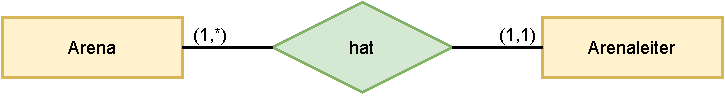
\includegraphics[width=0.7\linewidth]{includes/figures/example_entity_relationship_modell_min_max_one_to_many.pdf}
    \end{center}
\end{example}

\begin{example}{n:1 Relation (Min-Max-Notation)}
    In Pokémon ist jede \emph{Attacke} von genau einem \emph{Typ}.

    Natürlich können aber mehrere \emph{Attacken} auch vom gleichen \emph{Typ} sein.

    Damit gilt:
    \begin{center}
        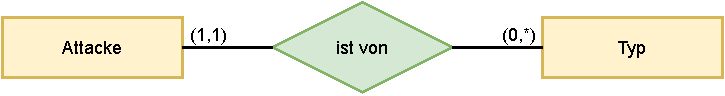
\includegraphics[width=0.7\linewidth]{includes/figures/example_entity_relationship_modell_min_max_many_to_one.pdf}
    \end{center}
\end{example}

\begin{example}{m:n Relation (Min-Max-Notation)}
    In Pokémon kann jedes \emph{Pokémon} einige \emph{Attacken} lernen.

    Die selbe \emph{Attacke} kann aber gleichzeitig von mehreren \emph{Pokémon} erlernt werden.

    Damit gilt:
    \begin{center}
        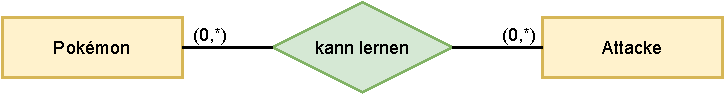
\includegraphics[width=0.7\linewidth]{includes/figures/example_entity_relationship_modell_min_max_many_to_many.pdf}
    \end{center}
\end{example}

\newpage
\subsubsection{UML-Notation}

\begin{defi}{UML-Notation}
    Die \emph{UML-Notation} ist eine Notation zur objektorientierten Modellierung.

    Bei den Kardinalitäten wird sich bezüglich der Reihenfolge bei der Chen-, bezüglich der Angaben bei der Min-Max-Notation bedient.
\end{defi}

\begin{defi}{Entität (UML-Notation)}
    \begin{wrapfigure}{r}{0.25\textwidth}
        \begin{center}
            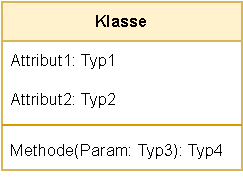
\includegraphics[width=0.2\textwidth]{includes/figures/definition_uml_entity.pdf}
        \end{center}
    \end{wrapfigure}
    Eine \emph{Entität} wird in der UML-Notation als Klasse dargestellt.
    Diese Klasse ist ein Rechteck mit drei Sektionen für
    \begin{itemize}
        \item den Klassennamen,
        \item Attribute (optional) und
        \item Methoden (optional).
    \end{itemize}
    Hierbei werden häufig nur die relevanten Details gezeigt.

    Die Notation ist wie folgt:
    \begin{center}
        \texttt{Sichtbarkeit: Name(Parameter): Rückgabetyp {Eigenschaften}}
    \end{center}

    Dabei gilt:
    \begin{itemize}
        \item Sichtbarkeiten:
              \begin{itemize}
                  \item \texttt{+}: public
                  \item \texttt{-}: private
                  \item \texttt{\#}: protected
              \end{itemize}
        \item Unterstrichene Attribute/Operationen stehen für Klassenattribute/Operationen
        \item Eigenschaften können Bedingungen (constraints) sein
        \item Schlüsselattribute z.B. als Kommentar / Eigenschaft
    \end{itemize}
\end{defi}

\begin{defi}{Relation (UML-Notation)}
    \begin{wrapfigure}{r}{0.65\textwidth}
        \begin{center}
            
\includegraphics[width=0.6\textwidth]{includes/figures/definition_uml_relation.pdf}
        \end{center}
    \end{wrapfigure}
    Für jeden an einer Relation beteiligten Entitätstyp $E_k$ wird angegeben, wie oft eine Entität minimal und maximal in $E_k$ enthalten sein darf, wenn der andere Eintrag ($n=2$) bzw. die anderen Einträge ($n>2$) fest gewählt ist, bzw. sind.

    Wir haben hier die gleiche Sichtweise wie bei der Chen-Notation, nur mit Angabe der minimalen und maximalen Elemente in der Entitätenmenge.

    Dadurch ist eine Angabe der Fälle
    \begin{itemize}
        \item \emph{optional}, wenn Kardinalität $= 0$, bzw.
        \item \emph{verpflichtend}, sonst.
    \end{itemize}

    Attributierte Relationen werden in der UML-Notation in einer assoziierten Klasse zusammengefasst.
\end{defi}

\newpage

\begin{example}{1:1 Relation (UML-Notation)}
    In Pokémon verleiht im Laufe des Spiels jede \emph{Arena} genau einen \emph{Orden}.

    Damit gilt:
    \begin{center}
        
\includegraphics[width=0.7\linewidth]{includes/figures/example_entity_relationship_modell_uml_one_to_one.pdf}
    \end{center}
\end{example}

\begin{example}{1:n Relation (UML-Notation)}
    In Pokémon hat jede \emph{Arena} mindestens einen, manchmal aber auch mehrere \emph{Arenaleiter}.

    Damit gilt:
    \begin{center}
        
\includegraphics[width=0.7\linewidth]{includes/figures/example_entity_relationship_modell_uml_one_to_many.pdf}
    \end{center}
\end{example}

\begin{example}{n:1 Relation (UML-Notation)}
    In Pokémon ist jede \emph{Attacke} von genau einem \emph{Typ}.

    Natürlich können aber mehrere \emph{Attacken} auch vom gleichen \emph{Typ} sein.

    Damit gilt:
    \begin{center}
        
\includegraphics[width=0.7\linewidth]{includes/figures/example_entity_relationship_modell_uml_many_to_one.pdf}
    \end{center}
\end{example}

\begin{example}{m:n Relation (UML-Notation)}
    In Pokémon kann jedes \emph{Pokémon} einige \emph{Attacken} lernen.

    Die selbe \emph{Attacke} kann aber gleichzeitig von mehreren \emph{Pokémon} erlernt werden.

    Damit gilt:
    \begin{center}
        
\includegraphics[width=0.7\linewidth]{includes/figures/example_entity_relationship_modell_uml_many_to_many.pdf}
    \end{center}
\end{example}

\begin{example}{UML-Relation mit Attributen}
    In Pokémon kann sich ein \emph{Pokémon} in teils mehrere \emph{Pokémon} entwickeln.

    Dabei sind verschiedene \emph{Bedingungen} zu erfüllen um diese Entwicklung zu erreichen.

    Damit gilt:
    \begin{center}
        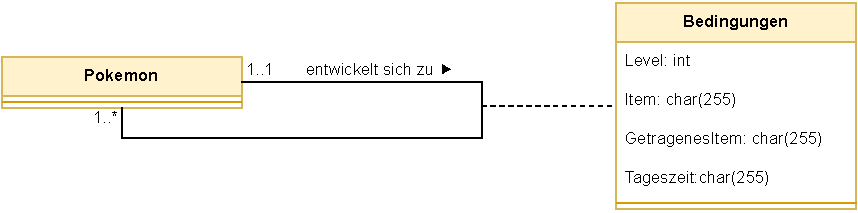
\includegraphics[width=0.7\linewidth]{includes/figures/example_uml_relation_associated.pdf}
    \end{center}
\end{example}

\begin{defi}{Vollständige und unvollständige UML-Relation}
    Eine UML-Relation heißt \emph{vollständig}, wenn alle Entitäten teilnehmen, \emph{unvollständig} sonst.

    In diesem Kontext werden oft Kurzformen genutzt:
    \begin{itemize}
        \item 0..* $\to$ *
        \item 1..1 $\to$ 1
        \item 1 als Default
    \end{itemize}

    Damit gilt:
    \begin{center}
        \begin{tabular}{cc}
            \underline{unvollständig}                                                                                   & \underline{vollständig}                                                                                   \\
            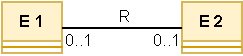
\includegraphics[width=0.4\textwidth]{includes/figures/definition_incomplete_uml_relation_one_to_one.pdf}   & 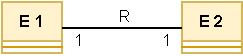
\includegraphics[width=0.4\textwidth]{includes/figures/definition_complete_uml_relation_one_to_one.pdf}   \\
            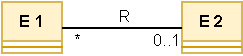
\includegraphics[width=0.4\textwidth]{includes/figures/definition_incomplete_uml_relation_many_to_one.pdf}  & 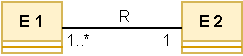
\includegraphics[width=0.4\textwidth]{includes/figures/definition_complete_uml_relation_many_to_one.pdf}  \\
            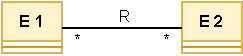
\includegraphics[width=0.4\textwidth]{includes/figures/definition_incomplete_uml_relation_many_to_many.pdf} & 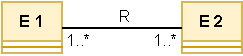
\includegraphics[width=0.4\textwidth]{includes/figures/definition_complete_uml_relation_many_to_many.pdf} \\
        \end{tabular}
    \end{center}
\end{defi}

\subsection{Generalisierung, Spezialisierung}

\begin{defi}{Generalisierungstyp}
    Der \emph{Generalisierungstyp} enthält die Attribute (Spalten), die alle spezialisierten Entitäten gemeinsam haben.

    Jede Entitätsmenge einer Generalisation verlangt eine eigenständige Tabelle, wobei der Primärschlüssel der übergeordneten Tabelle auch Primärschlüssel der untergeordneten Tabelle wird.

\end{defi}

\begin{defi}{Spezialisierungstyp}
    Die \emph{Spezialisierungstypen} enthalten die speziell für sie zutreffenden Attribute, wobei
    \begin{itemize}
        \item die Spezialisierung disjunkt oder überlappend sein kann und
        \item die Eigenschaften der Generalisierung erbt.
    \end{itemize}

    In einer spezialisierten Tabelle existieren keine Tupel, welche in der generalisierten Tabelle nicht vorkommen.
    Eine Spezialisierung wird durch Vererbung realisiert.

    Man beachte bei den Diagrammen:
    \begin{itemize}
        \item zeigt der Pfeil der Spezialisierung in Richtung \emph{der Generalisierung}, so ist sie \emph{nicht disjunkt}.
              \subitem \emph{Eselsbrücke}: Pfeile treffen sich $\to$ es existiert Schnittmenge $\to$ nicht disjunkt.
        \item zeigt der Pfeil der Spezialisierung in Richtung \emph{der Spezialisierung}, so ist sie \emph{disjunkt}.
              \subitem \emph{Eselsbrücke}: Pfeile treffen sich nie $\to$ es existiert keine Schnittmenge $\to$ disjunkt.
    \end{itemize}

    \begin{center}
        \begin{tabular}{ccc}
            \underline{nicht disjunkt} & \underline{disjunkt}                                              \\
            \\
            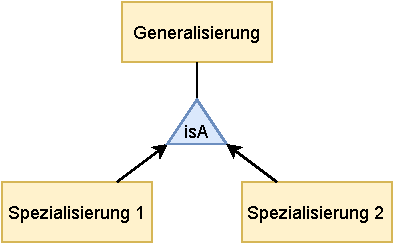
\includegraphics[width=0.3\textwidth]{includes/figures/definition_specialization_not_disjunct.pdf}
                                       & \quad                &
            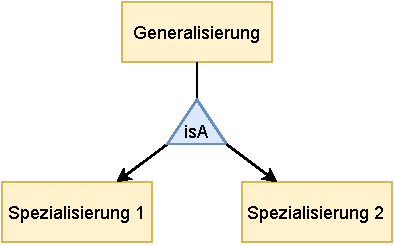
\includegraphics[width=0.3\textwidth]{includes/figures/definition_specialization_disjunct.pdf} \\
        \end{tabular}
    \end{center}

\end{defi}

\begin{example}{Spezialisierung}
    In Pokémon existieren \emph{keine} Pokémon mit der Typkombination Feuer und Pflanze.

    Damit gilt:
    \begin{center}
        \begin{tabular}{ccc}
            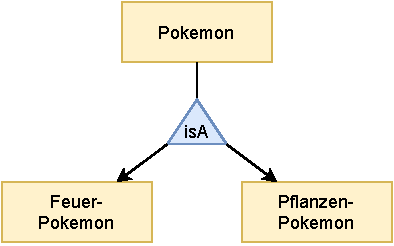
\includegraphics[width=0.4\linewidth]{includes/figures/example_specialization_er_diagram_disjunct.pdf}
             & \hspace{2em} &
            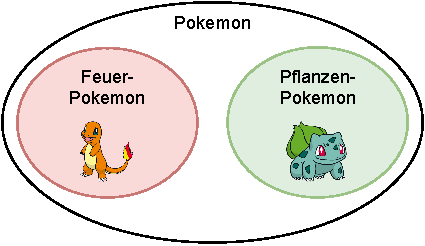
\includegraphics[width=0.4\linewidth]{includes/figures/example_specialization_venn_diagram_disjunct.pdf}
        \end{tabular}
    \end{center}

    Allerdings existieren Pokémon mit der Typkombination Wasser und Pflanze.

    Damit gilt:
    \begin{center}
        \begin{tabular}{ccc}
            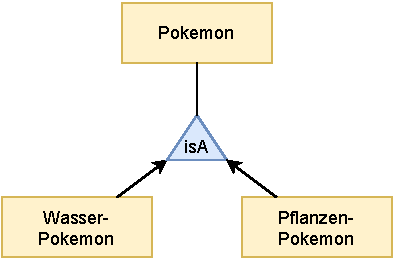
\includegraphics[width=0.4\linewidth]{includes/figures/example_specialization_er_diagram_not_disjunct.pdf}
             & \hspace{2em} &
            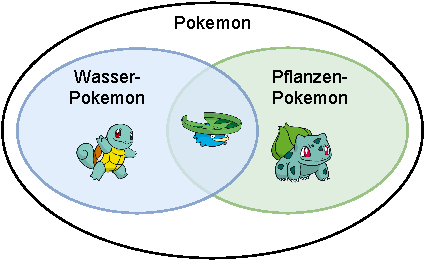
\includegraphics[width=0.4\linewidth]{includes/figures/example_specialization_venn_diagram_not_disjunct.pdf}
        \end{tabular}
    \end{center}
\end{example}

\subsection{Umsetzung von Relationen in RDBMS}

\begin{bonus}{1:1 Relation (RDBMS)}
    Eine Möglichkeit der Umsetzung ist über eine Fremdschlüsselbeziehung in einer der beiden Tabellen.

    Eine andere wäre über eine eigene Relationen-Tabelle.
    Hier darf aber dann jede Entität nur einmal vorkommen.
\end{bonus}

\begin{bonus}{n:1 Relation (RDBMS)}
    Eine Möglichkeit der Umsetzung sind zwei Tabellen für die Entitätstypen und die Realisierung der Relation als Fremdschlüssel in der Tabelle mit der $n$-Kardinalität.

    Eine andere Möglichkeit der Umsetzung sind zwei Tabellen für die Entitätstypen und eine eigene Tabelle für die Realisierung der Relation mit zwei Fremdschlüsseln.
\end{bonus}

\begin{bonus}{m:n Relation (RDBMS)}
    Die einzige Möglichkeit der Umsetzung sind zwei Tabellen für die Entitätstypen und eine eigene Tabelle für die Realisierung der Relation mit zwei Fremdschlüsseln.
\end{bonus}

\subsection{Relationales Modell}

\begin{defi}{Entitätstyp (Relationales Modell)}
    \begin{wrapfigure}{r}{0.425\textwidth}
        \begin{center}
            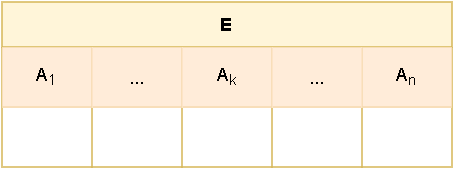
\includegraphics[width=0.375\textwidth]{includes/figures/definition_relational_modell_entity.pdf}
        \end{center}
    \end{wrapfigure}
    Ein wie bisher definierter Entitätstyp $E$ mit
    \[
        E: \{ A_1:D_1, \ldots, A_n:D_n \}
    \]
    wird im relationalen Modell zu einer \emph{Tabelle} $E$ mit:
    \begin{itemize}
        \item \emph{atomaren}\footnote{weder zusammengesetzt noch mehrwertig} Attributen $A_k$ als \emph{Spalten} mit Datentyp $D_k$
        \item Schlüsselattributen als \emph{primary keys}
    \end{itemize}

    Die Reihenfolge der Zeilen und Spalten ist nicht relevant.

    Enthaltene Informationen werden nur durch Datenwerte ausgedrückt.
\end{defi}

\begin{defi}{Schlüsselattribute}
    \begin{wrapfigure}{r}{0.5\textwidth}
        \begin{center}
            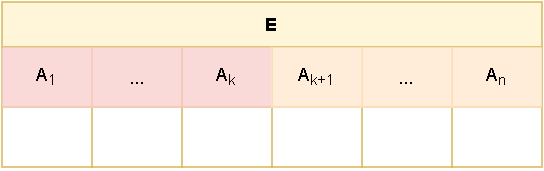
\includegraphics[width=0.45\textwidth]{includes/figures/definition_relational_modell_keys.pdf}
        \end{center}
    \end{wrapfigure}
    Jede Zeile bzw. Entität in der Tabelle $E$ beschreibt ein eindeutiges Objekt.

    Technisch sind Tabellen ohne Schlüsselattribut und Einträge, die in allen Werten identisch sind, denkbar, aber erst die Verwendung eindeutiger \emph{Schlüsselattribute} garantiert die Identifikation unterschiedlicher Objekte, selbst bei gleichen Werten der restlichen Attribute.

    Schlüsselattribute werden im relationalen Modell zu \emph{primary keys}.
\end{defi}

\begin{defi}{Zusammengesetzte Attribute (Relationales Modell)}
    \begin{wrapfigure}{r}{0.35\textwidth}
        \begin{center}
            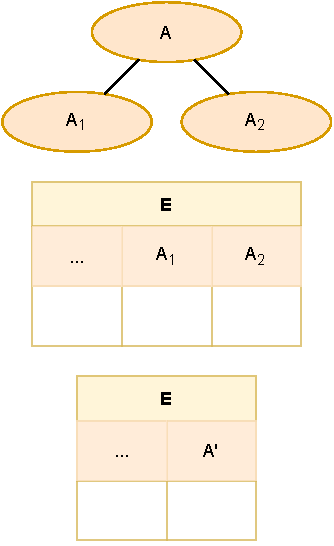
\includegraphics[width=0.3\textwidth]{includes/figures/definition_relational_modell_attribute_combined.pdf}
        \end{center}
    \end{wrapfigure}
    Bei einem zusammengesetzten Attribut $A$ mit
    \[
        A: [A_1 : D_1, \ldots, A_n:D_n]: D_1 \times \ldots \times D_n
    \]
    liegen die Informationen in den $A_k$, d.h. $A$ an sich enthält selbst keine Informationen.

    Deswegen kann das Modell in eine der zwei Möglichkeiten mit nur atomaren Attributen überführt werden:
    \begin{enumerate}
        \item \enquote{Umhängen} der Attribute $A_k$ direkt an den Entitätstypen
        \item Zusammenfassen der $A_k$ zu einem neuen gemeinsamen Attribut $A'$ (z.B. durch Stringkonkatenation)
    \end{enumerate}

    \vspace{6em}
\end{defi}

\begin{defi}{Mehrwertige Attribute (Relationales Modell)}
    \begin{wrapfigure}{r}{0.35\textwidth}
        \begin{center}
            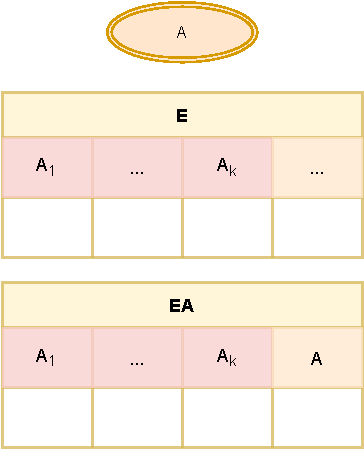
\includegraphics[width=0.3\textwidth]{includes/figures/definition_relational_modell_attribute_multiple.pdf}
        \end{center}
    \end{wrapfigure}
    Bei einem mehrwertigen Attribut $A$ werden die verschiedenen Ausprägungen von $A$ üblicher-weise in eine $1:n$-Relation mit einem weiteren Entitätstyp $E_A$ abgebildet.

    Eine allgemeinere Rolle von $E_A$ und eine entsprechende $m:n$-Relation ist auch denkbar.

    Schlüsselattribute von $E$ können so auch zu Schlüsselattributen von $E_A$ werden.
    Das hängt von der genauen Umsetzung der Relation ab.

    \vspace{6em}
\end{defi}

\begin{defi}{m:n Relation (Relationales Modell)}
    \begin{wrapfigure}{r}{0.575\textwidth}
        \begin{center}
            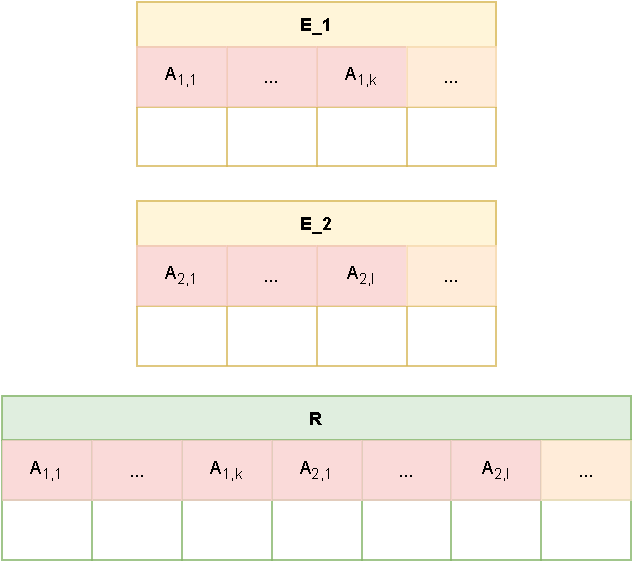
\includegraphics[width=0.525\textwidth]{includes/figures/definition_relational_modell_relation_many_to_many.pdf}
        \end{center}
    \end{wrapfigure}
    $n:m$-Relationen werden im relationalen Modell immer in einer eigenen Tabelle $R$ realisiert.

    Diese Tabelle $R$ enthält alle Schlüsselattribute der $E_k$, die vereint Schlüsselattribute von $R$ sind (\enquote{Fremdschlüssel}).
    Es ist aber auch möglich, ein künstliches Schlüsselattribut (meist \texttt{ID}) zu verwenden.

    Sollte $R$ attributiert sein, dann finden sich diese Attribute ebenfalls in $R$.

    \vspace{6em}
\end{defi}

\begin{defi}{1:n Relation (Relationales Modell)}
    \begin{wrapfigure}{r}{0.575\textwidth}
        \begin{center}
            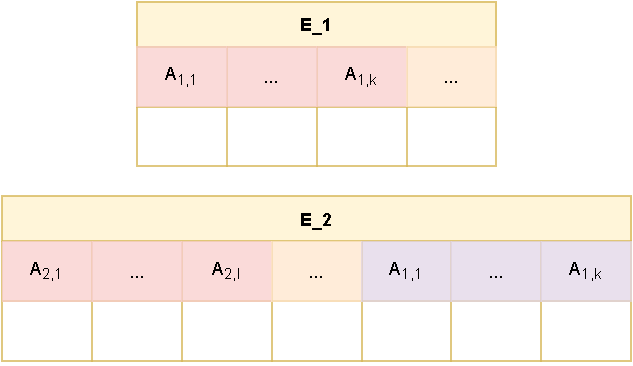
\includegraphics[width=0.525\textwidth]{includes/figures/definition_relational_modell_relation_one_to_many.pdf}
        \end{center}
    \end{wrapfigure}
    Da wir bei einer $1:n$-Relation eine partielle Funktion
    \[
        f: E_2 \to E_1
    \]
    haben, kann das Schlüsselattribut von $E_1$ als \enquote{Fremdschlüssel} in $E_2$ als weiteres Attribut eingebettet werden.
    Dort ist es kein Schlüssel von $E_2$, es referenziert nur die assoziierte Entität in $E_1$.\footnote{Der Fremdschlüssel kann nur in $E_2$, da man umgekehrt ein mehrwertiges Attribut in $E_1$ führen müsste, was im Widerspruch zur Atomarität stünde.}

    Sollte $E_1$ mehrere Schlüsselattribute haben, die den Primärschlüssel bilden, müssen selbstverständlich alle in $E_2$ vorkommen.
\end{defi}

\begin{defi}{1:1 Relation (Relationales Modell)}
    Bei einer $1:1$-Relation $R$ hat man jede der bisher benannten Möglichkeiten:
    \begin{enumerate}
        \item je eine Tabelle $E_1$ bzw. $E_2$ mit
              \begin{enumerate}
                  \item Fremdschlüssel in $E_1$
                  \item Fremdschlüssel in $E_2$
                  \item Fremdschlüssel in beiden Tabellen
              \end{enumerate}
        \item eine Tabelle $E'$ mit allen Attributen (Spalten) aus $E_1$ und $E_2$
        \item eine Tabelle für $R$ (analog zu $m:n$-Relation)
    \end{enumerate}

    Welche der Möglichkeiten am geeignetsten ist, ist am Ende von den Anforderungen und der Verwendung der Relation in der Praxis abhängig.
    Diese sind jeweils:

    \begin{enumerate}
        \item Daten aus $E_1$ und $E_2$ häufig gemeinsam benötigt und man sucht ein $e_2$ zu einem $e_1$, oder umgekehrt
        \item hebt zwar Trennung der modellierten Aspekte evtl. auf, kann aber sehr effizient sein
        \item zwar komplexer, aber stabil gegenüber Änderungen zu einer $1:n$- bzw. $m:n$-Relation
    \end{enumerate}

    \underline{Variante 1}
    \begin{center}
        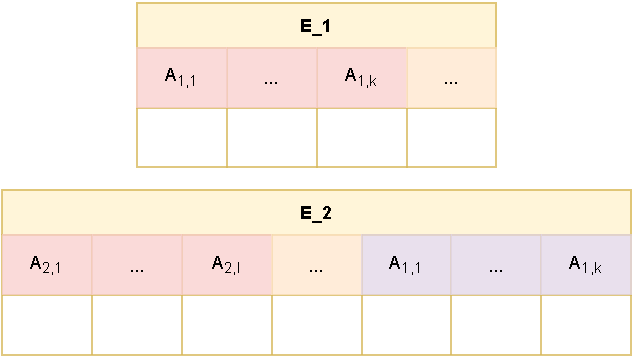
\includegraphics[width=0.525\textwidth]{includes/figures/definition_relational_modell_relation_one_to_one_1.pdf}
    \end{center}

    \underline{Variante 2}
    \begin{center}
        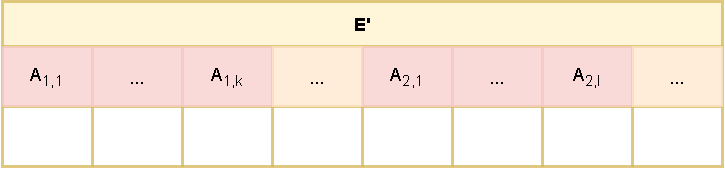
\includegraphics[width=0.6\textwidth]{includes/figures/definition_relational_modell_relation_one_to_one_2.pdf}
    \end{center}

    \underline{Variante 3}
    \begin{center}
        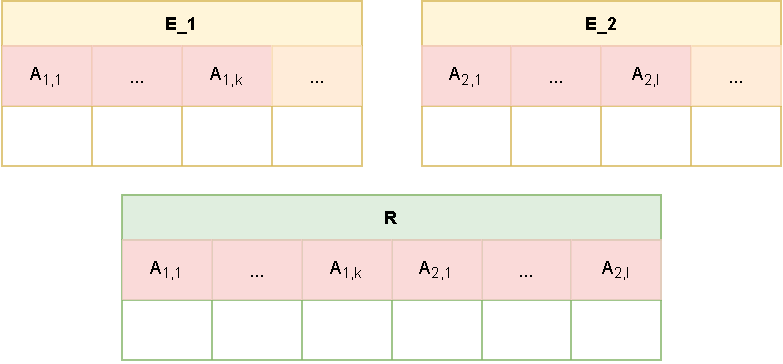
\includegraphics[width=0.675\textwidth]{includes/figures/definition_relational_modell_relation_one_to_one_3.pdf}
    \end{center}
\end{defi}